\hypertarget{performance-metrics-for-parallel-systems}{%
\section{Performance Metrics for Parallel
Systems}\label{performance-metrics-for-parallel-systems}}

\hypertarget{analytical-modeling}{%
\subsection{Analytical Modeling}\label{analytical-modeling}}

\begin{itemize}
\tightlist
\item
  Sequential Runtime

  \begin{itemize}
  \tightlist
  \item
    A sequential algorithm is evaluated by its runtime
  \end{itemize}
\item
  Parallel Runtime

  \begin{itemize}
  \tightlist
  \item
    The parallel runtime of a program depends on

    \begin{itemize}
    \tightlist
    \item
      the input size n,
    \item
      the number of processors p,
    \item
      and the communication parameters of the machine.
    \end{itemize}
  \item
    An algorithm must therefore be analyzed in the context of the
    underlying platform.
  \end{itemize}
\item
  Parallel System

  \begin{itemize}
  \tightlist
  \item
    A parallel system is a combination of a parallel algorithm and an
    underlying parallel platform.
  \end{itemize}
\item
  Wall-clock time

  \begin{itemize}
  \tightlist
  \item
    the time from the start of the first processor to the end of the
    last processor in a parallel ensemble
  \item
    in other words: the operation time of the processor which needs the
    most time
  \end{itemize}
\end{itemize}

\hypertarget{metrics}{%
\subsubsection{Metrics}\label{metrics}}

\begin{itemize}
\tightlist
\item
  $T_s(n)$: Zeitkomplexität des besten sequentiellen Vergleichalgorithmus
\item
  $T_p(p,n)$: Zeitkomplexität des besten parallelen Algorithmus
\item
  n: eindimensionale Inputgrösse
\item
  $p$: Anzahl ``Prozessoren'' (evtl. auch Threads, Cores, etc.)
\item
  Total Parallel Overhead $T_O = pT_P - T_S$
\item
  Speedup $S = T_S / T_P$
\item
  Speedup per processor = Efficiency $E = S / p = T_S / pT_P$
\end{itemize}

\hypertarget{speedup}{%
\subsubsection{Speedup}\label{speedup}}

\begin{itemize}
\tightlist
\item
  The lower bound of the speedup can be 0 (for parallel programs that
  never terminate)
\item
  The upper bound of the speedup should in theory be p, but in practice
  it is often lower than p.
\end{itemize}

\begin{figure}[H]
\centering
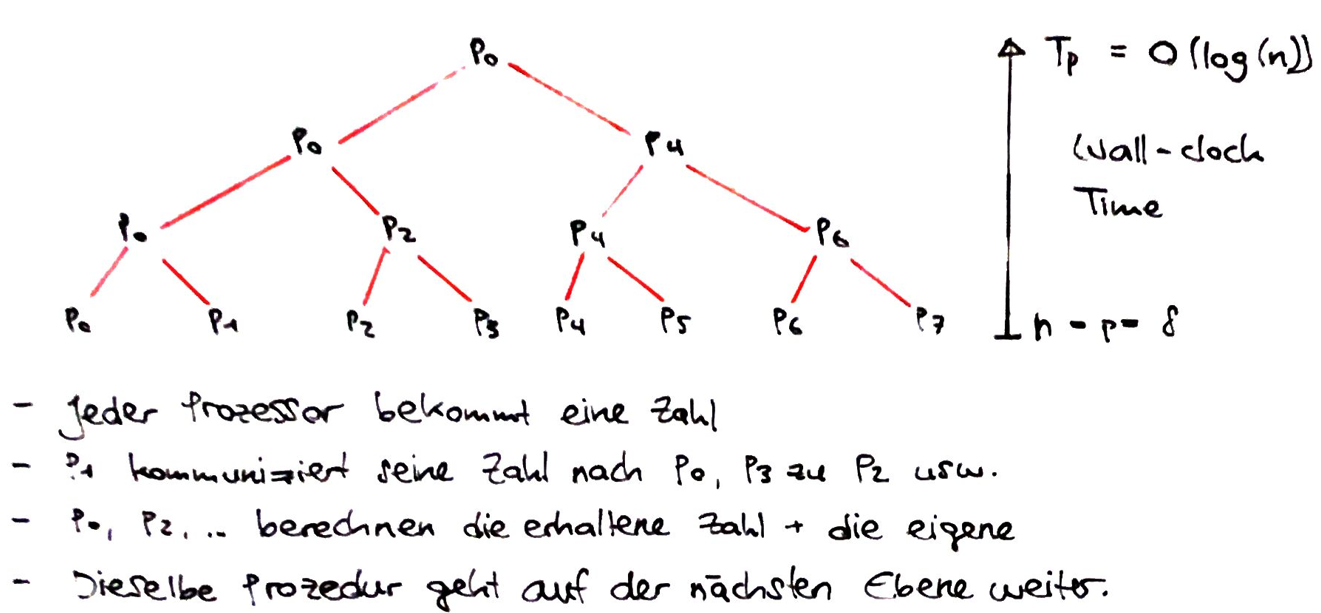
\includegraphics[width=0.7\textwidth]{figures/metricExample.png}
\caption{Metric Example}
\end{figure}

\hypertarget{big-o-landau-notation}{%
\subsubsection{Big-O / Landau Notation}\label{big-o-landau-notation}}

\begin{itemize}
\tightlist
\item
  $\mathcal{O}$ (Big O): Obergrenze, maximal so viele Schritte
\item
  $\Omega$ (Omega): Untergrenze, mindestens so viele Schritte
\item
  $\Theta$ (Theta): Obergrenze = Untergrenze, genau so viel
\end{itemize}

\hypertarget{cost-of-a-parallel-system}{%
\subsection{Cost of a Parallel System}\label{cost-of-a-parallel-system}}

\begin{itemize}
\tightlist
\item
  Cost (amount of total work)

  \begin{itemize}
  \tightlist
  \item
    is the product of parallel runtime and the number of processing
    elements used
  \item
    Cost $= p * T_P$
  \end{itemize}
\item
  Cost-Optimal System

  \begin{itemize}
  \tightlist
  \item
    a parallel system is said to be cost-optimal if the cost of solving
    a problem on a parallel computer is asymptotically identical to
    serial cost since $E = T_S / pT_P$, for cost-optimal systems: $E = \mathcal{O}(1)$
  \end{itemize}
\end{itemize}

\hypertarget{impact-of-non-cost-optimality}{%
\subsection{Impact of
Non-Cost-Optimality}\label{impact-of-non-cost-optimality}}

\begin{itemize}
\tightlist
\item
  The efficiency is calculated from the speedup over the number of
  processors (S/P)
\item
  Increasing the processors doesn't always solve the problem. Even if
  the speedup is increasing, the efficiency can shrink
\item
  speedup goes down as the problem size n is increased for a given p
\item
  efficiency doesn't depend on p, but goes down as the problem size is
  increased
\end{itemize}

\hypertarget{effect-of-granularity-on-performance}{%
\subsection{Effect of Granularity on
Performance}\label{effect-of-granularity-on-performance}}

\begin{figure}[H]
\centering
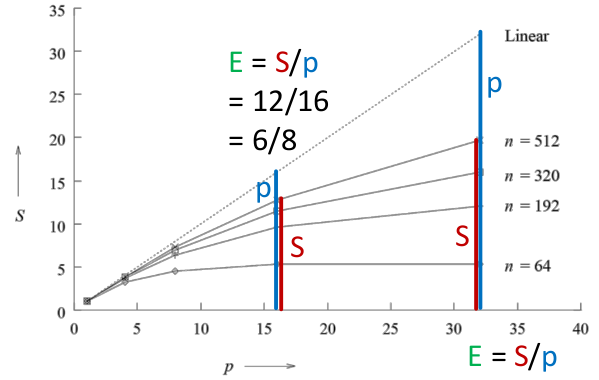
\includegraphics[width=0.7\textwidth]{figures/granularityOnPerformance.png}
\caption{Effect of Granularity on Performance}
\end{figure}

\begin{itemize}
\tightlist
\item
  Scaling-Down a parallel system is using fewer than the maximum
  possible number of processing elements to execute a parallel algorithm
\item
  This often improves the efficiency
\item
  One way of scaling down could be

  \begin{itemize}
  \tightlist
  \item
    think of each processor in the original case as a virtual processor
    and to assign virtual processors equally to scaled down processors
  \item
    since the number of processing elements decreases by a factor of
    $n/p$, the computation at each processing element increases by a
    factor of $n/p$
  \end{itemize}
\end{itemize}

\clearpage